\documentclass[11pt]{article}

% some definitions for the title page
\newcommand{\reporttitle}{Image Registration}
\newcommand{\reportdescription}{This week's lecture contains content about image registration and how we can `combine' two images of the same object together with transformations. This week's paper recommendation is~\cite{jaderberg2016spatial}}

% load some definitions and default packages
%---------------------------------------------------------------------------
%	PACKAGES AND OTHER DOCUMENT CONFIGURATIONS
%---------------------------------------------------------------------------

\usepackage[twoside]{fancyhdr}
\usepackage{csquotes}

\usepackage[a4paper,hmargin=2.0cm,vmargin=1.0cm,includeheadfoot]{geometry}
% \usepackage{natbib} % for bibliography
\usepackage{biblatex}
\usepackage{tabularx,longtable,multirow,subfigure,caption}%hangcaption
\usepackage{fancyhdr} % page layout
\usepackage{url} % URLs
\usepackage[english]{babel}
\usepackage{amsmath}
\usepackage{graphicx}
\usepackage{dsfont}
\usepackage{epstopdf} % automatically replace .eps with .pdf in graphics
% \usepackage{backref} % needed for citations
\usepackage{array}
\usepackage{latexsym}
\usepackage[pdftex,hypertexnames=false,colorlinks]{hyperref} % provide links in pdf (had pagebackref)
\usepackage{booktabs}
\usepackage{wrapfig}
\usepackage{caption}  % Required for \captionof
\usepackage{float} % for H option in figures
\usepackage{amssymb}
\usepackage{amsmath}
\usepackage[nottoc]{tocbibind}

%%% Default fonts
\renewcommand*{\rmdefault}{bch}
\renewcommand*{\ttdefault}{cmtt}

%%% Default settings (page layout)
\setlength{\parindent}{0em}  % indentation of paragraph
\setlength{\parskip}{.3em}

\setlength{\headheight}{14.5pt}
\pagestyle{fancy}

\fancyfoot[ER,OL]{\thepage}%Page no. in the left on odd pages and on right on even pages

\fancyfoot[OC,EC]{\sffamily }
\renewcommand{\headrulewidth}{0.1pt}
\renewcommand{\footrulewidth}{0.1pt}
\captionsetup{margin=10pt,font=small,labelfont=bf}
% Here, you can define your own macros. Some examples are given below.

\newcommand{\R}[0]{\mathds{R}} % real numbers
\newcommand{\Z}[0]{\mathds{Z}} % integers
\newcommand{\N}[0]{\mathds{N}} % natural numbers
\newcommand{\C}[0]{\mathds{C}} % complex numbers
\renewcommand{\vec}[1]{{\boldsymbol{{#1}}}} % vector
\newcommand{\mat}[1]{{\boldsymbol{{#1}}}} % matrix

\usepackage{pifont,mdframed}
\newenvironment{warning}
  {\par\begin{mdframed}[linewidth=1pt,linecolor=black]%
    \begin{list}{}{\leftmargin=1cm
                   \labelwidth=\leftmargin}\item[\Large\ding{43}]}
  {\end{list}\end{mdframed}\par}

\bibliography{../bibliography}

\begin{document}

% Include the title page
\begin{titlepage}

    \newcommand{\HRule}{\rule{\linewidth}{0.5mm}} % Defines a new command for the horizontal lines, change thickness here
    
    \center % Center everything on the page
     
    %------------------------------------------------------------------------
    %	HEADING SECTIONS
    %------------------------------------------------------------------------
    
    \textsc{\Large Department of Computing}\\[0.5cm] 
    \textsc{\large Imperial College of Science, Technology and Medicine}\\[0.5cm] 
    
    %------------------------------------------------------------------------
    %	TITLE SECTION
    %------------------------------------------------------------------------
    
    \HRule \\[0.4cm]
    { \huge \bfseries \reporttitle}\\ % Title of your document
    \HRule \\[0.4cm]

    \textit{\reportdescription}
    
    \vspace{2em}

    %------------------------------------------------------------------------
    %	AUTHOR SECTION
    %------------------------------------------------------------------------
    
    \large \emph{Author: Anton Zhitomirsky}

    \vspace{1em}

    \global\let\newpagegood\newpage
    \global\let\newpage\relax
    
\end{titlepage}

\global\let\newpage\newpagegood

\tableofcontents

\clearpage

\section{Image Registration}

\begin{figure}[H]
    \centering
    \fbox{\includegraphics[page=3, trim=2cm 3cm 1cm 6.5cm, clip=true, width=.9\linewidth]{03 - Image Registration.pdf}}
\end{figure}

We typically don't know the analytical value of $f$, however, we have it in a sampled manner. 

If we have an image of a patient, with two different imaging modalities to scan the same plane, we require image registration to see how does a pixel look like in another image. This requires a spatial transformation between the two images. 

\begin{equation*}
    \begin{pmatrix}
        x' \\ y'
    \end{pmatrix}
    =
    T 
    \begin{pmatrix}
        x \\ y
    \end{pmatrix} \quad \text{where $T$ is the transform operation from one image to another}
\end{equation*}

\subsection{Coordinate systems and transformations}

\begin{figure}[H]
    \centering
    \subfigure[Image coordinate system]{
        \fbox{\includegraphics[page=6, trim=9cm 3.5cm 9cm 8.8cm, clip=true, width=.45\linewidth]{03 - Image Registration.pdf}}\label{fig:image-coordinate-system}
    }
    \subfigure[Word coordinate system]{
        \fbox{\includegraphics[page=7, trim=8.8cm 3.5cm 9cm 7.7cm, clip=true, width=.45\linewidth]{03 - Image Registration.pdf}}\label{fig:world-coordinate-system}
    }
\end{figure}

In an image coordinate system in Figure~\ref{fig:image-coordinate-system} we have a pixel grid of a set width and height. Each pixel has a certain physical dimension, which is obtained form the measurement device. This assumes that the x and y axis is aligned with the pixel grid lines. Typically this is not the case.

Therefore, we introduce the real-world coordinate system in Figure~\ref{fig:world-coordinate-system}. Here, it is not necessarily aligned with the x and y, and the origin is not necessarily at (0,0). (We don't really worry when it comes to segmentation but when we relate images together then it becomes as concern because they may be scanned at different transformations). In cartesian space, you worry about the orthogonal unit vectors defining the directions and the origin. 

\begin{equation*}
    \begin{pmatrix}
        X \\ Y \\ 1
    \end{pmatrix}
    =
    \underbrace{
        \overbrace{
        \begin{bmatrix}
            1 & 0 & \color{red}ox \\ 
            0 & 1 & \color{red}oy \\
            0 & 0 & 1 
        \end{bmatrix}
        }^\text{translation vectors}    
        \overbrace{
            \begin{bmatrix}
                \color{violet}dxx & \color{violet}dyx & 0 \\ 
                \color{violet}dxy & \color{violet}dyy & 0 \\
                0 & 0 & 1 
            \end{bmatrix}
        }^\text{direction vectors}    
        \overbrace{
            \begin{bmatrix}
                \color{green}sx & 0 & 0 \\ 
                0 & \color{green}sy & 0 \\
                0 & 0 & 1 
            \end{bmatrix}
        }^\text{scaling matrix}
    }_{T_{ItW}}    
    \begin{pmatrix}
        x \\ y \\ 1
    \end{pmatrix} 
\end{equation*}

This \textbf{affine} transformation equation uses homogeneous coordinates\footnote{TODO}. We write them in a 3D form, because we can model interesting geometric rtasnformations such as translations. 

\begin{itemize}
    \item \textbf{translation vectors}: translation from the origin of the world coordinates to the origin of the image coordinates
    \item \textbf{direction vectors}: define the directions on the axis of the image
    \item \textbf{scaling matrix}: defines the pixel spacing to produce a scaled version of the image or the image coordinates in the X and Y direction.
\end{itemize}

Therefore, if we have more than one world, A and B and we wish to align them, first by aligning the world coordinates then doing the remaining transformations.

\begin{equation*}
    \begin{pmatrix}
        x_A \\ y_A
    \end{pmatrix}
    =
    T^A_{WtI} T_{BtA} T^B_{ItW}
    \begin{pmatrix}
        x_B \\ y_B
    \end{pmatrix}
\end{equation*}

Image transformation is about finding $T_{BtA}$, since the other transformations can be obtained from the measurement devices.

\section{Transformation Models}

\begin{figure}[H]
    \centering
    \fbox{\includegraphics[page=15, trim=4cm 3cm 4cm 6.6cm, clip=true, width=.7\linewidth]{03 - Image Registration.pdf}}\label{fig:transformation-models}
\end{figure}

\subsection{Linear Transformations}

\subsubsection{Rigid}

Allows for rotation and translation. It is useful in the real world because it can't scale, mimmiking real-world; distances are always maintained. 

\begin{minipage}[c]{0.5\linewidth}
    \begin{equation*}
        T= \begin{bmatrix}
            1 & 0 & \color{red}t_x \\ 
            0 & 1 & \color{red}t_y \\ 
            0 & 0 & 1
        \end{bmatrix}
    \end{equation*}
\end{minipage}\hfill
\begin{minipage}[c]{0.5\linewidth}
    \begin{figure}[H]
        \centering
        \fbox{\includegraphics[page=16, trim=2cm 4cm 22.5cm 13cm, clip=true, width=.5\linewidth]{03 - Image Registration.pdf}}
        \caption*{Translation}
    \end{figure}
\end{minipage}

\begin{minipage}[c]{0.5\linewidth}
    \begin{equation*}
        R = \begin{bmatrix}
            \cos \color{red}{\theta} & \sin \color{red}{\theta} & 0 \\ 
            -\sin \color{red}{\theta} & \cos \color{red}{\theta} & 0 \\ 
            0 & 0 & 1
        \end{bmatrix}
    \end{equation*}
\end{minipage}\hfill
\begin{minipage}[c]{0.5\linewidth}
    \begin{figure}[H]
        \centering
        \fbox{\includegraphics[page=16, trim=10cm 4cm 16.5cm 13cm, clip=true, width=.3\linewidth]{03 - Image Registration.pdf}}
        \caption*{Rotation}
    \end{figure}
\end{minipage}

\subsubsection{Similarity}

Allows for scaling, which is a similarity transform

\begin{minipage}[c]{0.5\linewidth}
    \begin{equation*}
        S = \begin{bmatrix}
            \color{red}{s_x} & 0 & 0 \\ 
            0 & \color{red}{s_y} & 0 \\ 
            0 & 0 & 1
        \end{bmatrix}
    \end{equation*}
\end{minipage}\hfill
\begin{minipage}[c]{0.5\linewidth}
    \begin{figure}[H]
        \centering
        \subfigure{
            \fbox{\includegraphics[page=22, trim=16cm 4.5cm 9.5cm 14cm, clip=true, width=.4\linewidth]{03 - Image Registration.pdf}}
        }
        \caption*{Shearing}
    \end{figure}
\end{minipage}

\subsubsection{Affine}

Allows for scaling in different dimensions, and shears. They allow for scaling in different directions. No matter what affine transformation you do, lines will always be parallel.

Shearing is achieved by doing a combination of different transformation matricies, specifically $RSR^{-1}$; a rotation, scaling and rotation.

\begin{equation*}
    S = \begin{bmatrix}
        \cos \color{red}{\omega} & \sin \color{red}{\omega} & 0 \\ 
        -\sin \color{red}{\omega} & \cos \color{red}{\omega} & 0 \\ 
        0 & 0 & 1
    \end{bmatrix}
\end{equation*}

\begin{figure}[H]
    \centering
    \subfigure{
        \fbox{\includegraphics[page=18, trim=23.3cm 3.5cm 2cm 13cm, clip=true, width=.15\linewidth]{03 - Image Registration.pdf}}
    }
    \subfigure{
        \fbox{\includegraphics[page=19, trim=23.3cm 3.5cm 2cm 13cm, clip=true, width=.15\linewidth]{03 - Image Registration.pdf}}
    }
    \subfigure{
        \fbox{\includegraphics[page=20, trim=23.3cm 3.5cm 2cm 13cm, clip=true, width=.15\linewidth]{03 - Image Registration.pdf}}
    }
    \subfigure{
        \fbox{\includegraphics[page=21, trim=23.3cm 3.5cm 2cm 13cm, clip=true, width=.15\linewidth]{03 - Image Registration.pdf}}
    }
    \subfigure{
        \fbox{\includegraphics[page=22, trim=23.3cm 3.5cm 2cm 13cm, clip=true, width=.15\linewidth]{03 - Image Registration.pdf}}
    }
    \caption*{Shearing}
\end{figure}

\subsubsection{Combinations of Linear Transformations}

The nice thing about linear transformations is that you can combine them all together into one big matrix and then directly operate on the matrix coeffiecients.

\subsection{Non-Linear (Free-form) Transformations}

\subsubsection{Control Point Based Model}

Free-form transformations; lines can cross (in topology preserving transformations this cannot happen)

\begin{figure}[H]
    \centering
    \fbox{\includegraphics[page=24, trim=4cm 5cm 2cm 9cm, clip=true, width=\linewidth]{03 - Image Registration.pdf}}
\end{figure}

\begin{enumerate}
    \item We can embed an image onto a grid (not a pixel grid)
    \item We prescribe the motion/deformation at each grid point. These are control points. The blue arrows prescribe how the trainsformation at that point should behave in a smooth fashion.
    \item The underlying blue grid comes out smooth despite ugly red grid.
    \item This is because we start interpolating between the deformation values to produce a smooth deformation.
    \item This model is based on linear-interpolation, where the (triangle) functions have the directions applied to them, and the deformations are applied linearly.
\end{enumerate}

There are also finite-element methods, and dense displacement fields (we assign a direction for each pixel).

\subsection{Applications}

\begin{figure}[H]
    \centering
        \fbox{\includegraphics[page=27, trim=2cm 7cm 2.8cm 9cm, clip=true, width=\linewidth]{03 - Image Registration.pdf}}
    \caption*{(left) Satelite Imaging (right) Point Correspondences}
\end{figure}

\begin{figure}[H]
    \centering
    \fbox{\includegraphics[page=28, trim=2cm 7cm 2.8cm 9cm, clip=true, width=\linewidth]{03 - Image Registration.pdf}}
    \caption*{Panoramic Image Stitching}
\end{figure}

\begin{figure}[H]
    \centering
    \fbox{\includegraphics[page=29, trim=4cm 3cm 2cm 9cm, clip=true, width=\linewidth]{03 - Image Registration.pdf}}
    \caption*{Optical Flow (3D reconstructions)}
\end{figure}

\subsection{Medical Applications}

\begin{itemize}
    \item Cardiac Motion tracking
    \item Respiration Motion tracking
    \item Multi-modal Image Fusion
    \item Pre- and Post-op comparison
\end{itemize}

\subsubsection{Intra-subject Registration}

Perform Atlas construction: assuming you have different picutres of the human brain, you would like to find out what the average brain looks like, by integrating and averaging all images together. 

\begin{figure}[H]
    \centering
    \fbox{\includegraphics[page=36, trim=1cm 3.5cm 1cm 7cm, clip=true, width=\linewidth]{03 - Image Registration.pdf}}
    \caption*{Atlas Iterations: Step 1 | Rigid}
\end{figure}

\begin{figure}[H]
    \centering
    \fbox{\includegraphics[page=37, trim=1cm 3.5cm 1cm 7cm, clip=true, width=\linewidth]{03 - Image Registration.pdf}}
    \caption*{Atlas Iterations: Step 2 | Affine}
\end{figure}

\begin{figure}[H]
    \centering
    \fbox{\includegraphics[page=38, trim=1cm 3.5cm 1cm 7cm, clip=true, width=\linewidth]{03 - Image Registration.pdf}}
    \caption*{Atlas Iterations: Step 3 | Nonrigid}
\end{figure}

\section{Intensity-based image registration}

Assumption: When images are correctly aligned they should look very similar.

The estimation of transformation parameters is driven by the appearance of the images, and images are registered when they appear similar.

\begin{figure}[H]
    \centering
    \fbox{\includegraphics[page=50, trim=4.7cm 5cm 5cm 7cm, clip=true, width=\linewidth]{03 - Image Registration.pdf}}
    \caption*{Pixel differences before registration (left) and after (right)}
\end{figure}

\subsection{Components}

\subsubsection{Objective Function}

\begin{equation}
    C(T) = D(I \circ T, J)
\end{equation}

\begin{itemize}
    \item $T$: Transformation
    \item $D$: Dissimilarity measure
    \item $I\circ T$: Moving Image
    \item $J$: Fixed Image
\end{itemize}

\subsubsection{Optimisation Problem}

\begin{equation}
    \hat T = \arg \min_T C(T)
\end{equation}

\begin{itemize}
    \item $\arg$: return the argument (not the value)
    \item $\min_T$: search $T$ with minimum cost value
    \item $C(T)$: cost function where $C:\mathbb R^d \rightarrow \mathbb R$ where $d$ is the d.o.f/ parameters of transform.
\end{itemize}

\subsection{Mono-modal Registration}

Image intensities are related by a (simple) function. Here, a simple difference may be sufficient.

Assumption: the identity relationship between intensity distributions (``images should be ideally matched after registraition'').  

\subsubsection{Sum of squared differences}

\begin{equation}
    D_{SSD}(I \circ T,J) = \frac 1 N  \sum^N_{i=1} (I(T(x_i))-J(x_i))^2
\end{equation}

\subsubsection{Sum of absolute differences}

\begin{equation}
    D_{SAD}(I \circ T,J) = \frac 1 N  \sum^N_{i=1} |I(T(x_i))-J(x_i)|
\end{equation}

\subsubsection{Correlation coefficient (CC)}

With the above dissimilarity measure, there are some scenarios where that's not quite the case. For example, if the brightness changes, then subtraction is not a good metric. We can instead compute the normalised corss correlation betwen the pixel values or the pixel intensities in one image and in the second image. We get values between 0 (no correlation) and 1 (perfect correlation).

\begin{equation}
    D_{CC}(I \circ T,J)=-\frac{
\overbrace{
   \frac{1}{N} \sum^N_{i=1}(I(T(x_i))-\mu_I)(J(x_i)-\mu_I)
}^{cov(I,J)}
}{
\underbrace{
\sqrt{\frac 1 N \sum^N_{i=1}(I(T(x_i))-\mu_I)^2
}
}_{\sigma_I}
\underbrace{
\sqrt{\frac 1 N \sum^N_{i=1}(J(x_i)-\mu_J)^2
}
}_{\sigma_I}
}
\end{equation}

\begin{figure}[H]
    \centering
    \fbox{\includegraphics[page=55, trim=2.5cm 8cm 1cm 3cm, clip=true, width=\linewidth]{03 - Image Registration.pdf}}
\end{figure}

Assumption: Linear relaionship betwene intensity distribution.

\subsection{Multi-modal Registration}

Image intensities are related by a complex funciton or statistical relationship

\begin{figure}[H]
    \centering
    \fbox{\includegraphics[page=56, trim=2.5cm 2.7cm 5cm 6.3cm, clip=true, width=.55\linewidth]{03 - Image Registration.pdf}}
    \caption*{Dissimiarity in the case where images look different (posisbly different modalities) to do registration we may find correspondences (red arrows).}
\end{figure}

However, it may be that the images have very different behaviours in the two images (tumor isn't visible in one of the imaging modalities).

\subsubsection{Statistical Relationship | Intesntiy Histograms}

\begin{figure}[H]
    \centering
    \fbox{\includegraphics[page=57, trim=4.3cm 3.5cm 6.5cm 7.1cm, clip=true, width=.5\linewidth]{03 - Image Registration.pdf}}
    \caption*{Cluster all pixels in a histograms. If two images are perfectly aligned, then this is fairly clustered, otherwise, the two images are completely misaligned.}
\end{figure}

\begin{figure}[H]
    \centering
    \fbox{\includegraphics[page=58, trim=4.6cm 5.3cm 5cm 8cm, clip=true, width=.6\linewidth]{03 - Image Registration.pdf}}
    \caption*{Theoretical Example: (left) perfectly registered, the entire histogram is aligned along the diagonal (pixel values are exactly equivalent between the two), (middle) by shifting, we often have the same value but not all the time.}
\end{figure}

\begin{figure}[H]
    \centering
    \subfigure{
        \fbox{\includegraphics[page=59, trim=19.5cm 14.6cm 4.5cm 3.3cm, clip=true, width=.46\linewidth]{03 - Image Registration.pdf}}
    }
    \subfigure{
        \fbox{\includegraphics[page=60, trim=19.5cm 14.6cm 4.5cm 3.3cm, clip=true, width=.46\linewidth]{03 - Image Registration.pdf}}
    }
    \subfigure[Comparison between CT and MR scan]{
        \fbox{\includegraphics[page=59, trim=4.6cm 5.3cm 5cm 8cm, clip=true, width=.46\linewidth]{03 - Image Registration.pdf}}
    }
    \subfigure[Comparison between MR and PET scan]{
        \fbox{\includegraphics[page=60, trim=4.6cm 5.3cm 5cm 8cm, clip=true, width=.46\linewidth]{03 - Image Registration.pdf}}
    }
\end{figure}

\subsubsection{Intensity Distribution}

\begin{figure}[H]
    \centering
    \fbox{\includegraphics[page=61, trim=17.3cm 9cm 4.7cm 4.5cm, clip=true, width=.3\linewidth]{03 - Image Registration.pdf}}
\end{figure}

\begin{equation}
    p(i,j)=\frac {h(i,j)} N
\end{equation}

joint probability of an image point having a value $i$ in an image $I$  and value $j$ in image $J$, where $h(\cdot, \cdot)$ is the counts in histogram.

\begin{equation}
    p(i) = \sum_j p(i,j)
\end{equation}

marginal probability of an image point having a value $i$ in image $I$.

\begin{equation}
    p(j) = \sum_i p(i,j)
\end{equation}

marginal probability of an image point having a value $j$ in image $J$.

\subsubsection{Shannon entropy}

\begin{equation}
    H(I) = - \sum_i p(i)\log p(i)
\end{equation}

amount of arbitraty information contained in image $I$. This value is low if every pixel has the same pixel intensity value or high if there is a lot of infromation.

\subsubsection{Joint entropy}

\begin{equation}
    H(I,J) = - \sum_i \sum_j p(i,j)\log p(i,j)
\end{equation}

amount of information contained in the combined image $I,J$.

This could be used for image registration: ``it measures how clustered a space is, and minimising that entropy is a good criterium is good for image registration'' $D_{JE}(I\circ T, J) = H(I \circ T, J)$.

\subsubsection{Mutual infromation}

\begin{equation}
    MI(I,J) = H(I) + H(J) - H(I,J)
\end{equation}

describes how well one image can be explined by another image. This can be rewritten in terms of a marginal and join probabilities:

\begin{equation}
    MI(I,J) = \sum_i \sum_j p(i,j)\log \frac{p(i,j)}{p(i)p(j)}
\end{equation}

Where the dissimilaity measure is redefined as

\begin{equation}
    D_{MI}(I\circ T,J)=-MI(I \circ T, J)
\end{equation}

\subsubsection{Normalised mutual information}

\begin{equation}
    NMI(I,J) = \frac{H(I) + H(J)}{H(I,J)}
\end{equation}

is independent of the amount of overlap bewteen images. The dissimilarity measure is redefined as 

\begin{equation}
    D_{MI}(I\circ T,J)=-NMI(I \circ T, J)
\end{equation}

Assumption: statistical relationship between intensity distributions

\subsection{Conclusion}

\begin{figure}[H]
    \centering
    \fbox{\includegraphics[page=65, trim=4cm 5cm 4cm 9.5cm, clip=true, width=.9\linewidth]{03 - Image Registration.pdf}}
\end{figure}

\begin{figure}[H]
    \centering
    \fbox{\includegraphics[page=66, trim=4cm 5cm 4cm 9.5cm, clip=true, width=.9\linewidth]{03 - Image Registration.pdf}}
\end{figure}

Here we see that $NMI$ is the best for multi-modal. It doesn't assume that one image is brighter, but measures when are these two images maximally statistically related. 

\subsubsection{Image Overlap}

(Dis)similarity mesaures are evaluated in the overalpping region of two images, which therefore requires a capture range evaluation.

\begin{figure}[H]
    \centering
    \fbox{\includegraphics[page=68, trim=6.5cm 5cm 6.5cm 7.5cm, clip=true, width=.9\linewidth]{03 - Image Registration.pdf}}
    \caption*{Optimisation strategy needed: need to minimise cost function, you may find local minimums, which may be a problem.}
\end{figure}

You therefore try to combat this by using:

\begin{itemize}
    \item Multi-resolution strategies | Successsively increase degrees of freedom
    \item smoothing | Gaussian image pyramids
\end{itemize}

\subsubsection{Interpolation}

\begin{figure}[H]
    \centering
    \fbox{\includegraphics[page=71, trim=2cm 3.5cm 2cm 5.8cm, clip=true, width=.9\linewidth]{03 - Image Registration.pdf}}
    % \caption*{}
\end{figure}

Quite often, interpolation is needed, because pixel grids aren't aligned. But still, you need to compare intensities, therefore use linear interpolations for pixel comparisons.

\subsubsection{Registration as an Iterative Process}

\begin{figure}[H]
    \centering
    \fbox{\includegraphics[page=73, trim=4.5cm 3.5cm 4.5cm 6cm, clip=true, width=.9\linewidth]{03 - Image Registration.pdf}}
    \caption*{Optimisation stragecy: gradient based, e.g. stochastic or complete gradient descent (without subsampling)}
\end{figure}

\subsubsection{Optimisation strategies}

\begin{itemize}
    \item Gradient-descent
    \item stochastic Optimisation
    \item bayesian Optimisation
    \item discrete Optimisation
    \item convex Optimisation
    \item downhill-simplex
    \item \dots
\end{itemize}

\section{Neural networks for image registration | Supervised}

\subsection{FlowNet}

Supervised Learning approach.

\begin{figure}[H]
    \centering
    \fbox{\includegraphics[page=77, trim=3cm 4cm 3cm 8.5cm, clip=true, width=.9\linewidth]{03 - Image Registration.pdf}}
    % \caption*{}
\end{figure}

Take two frames of a video and put them into a CNN architecture. The idea is to predict the dense displacement fields between the two video frames. How do you train this?

\begin{figure}[H]
    \centering
    \fbox{\includegraphics[page=78, trim=3cm 6.5cm 3cm 8.5cm, clip=true, width=.9\linewidth]{03 - Image Registration.pdf}}
    % \caption*{}
\end{figure}

The network proposed is the first paper to do registration in neural networks. There are 6 channels because $2\times 3$ RGB channels, then you contract them in the network and predict the output. 

\begin{figure}[H]
    \centering
    \fbox{\includegraphics[page=79, trim=3cm 5.5cm 3cm 8.5cm, clip=true, width=.9\linewidth]{03 - Image Registration.pdf}}
    % \caption*{}
\end{figure}

Alternative architecture | network has two separate CNNs for both frames. Then do a pixel-wise correlation betwen the features then pass them through the network predicing the output. Here, we explicitly calculate a correlation between the features in both the video frames.

\begin{figure}[H]
    \centering
    \fbox{\includegraphics[page=80, trim=3cm 4cm 3cm 8.5cm, clip=true, width=.9\linewidth]{03 - Image Registration.pdf}}
    % \caption*{}
\end{figure}

Lastly, there is an upsampling to estimate pixel-wise dense displacement.

\subsubsection{How to train such a network?}

Key requirement, is that you need to know the ground-truth of the optical flow. In the real-world scenario, you need to take real videos, then they renderred flying chairs in different viewpoints into these videos. Because these are rendered, you know the geometric trasnformation.

\subsection{FlowNet 2.0}

Evolution of Optical Flow Estimation with Deep networks

\begin{figure}[H]
    \centering
    \fbox{\includegraphics[page=86, trim=2cm 3cm 1cm 7.8cm, clip=true, width=.9\linewidth]{03 - Image Registration.pdf}}
    % \caption*{}
\end{figure}

Take the flow correlation network (not good for large displacements), build a new architecture:

\begin{enumerate}
    \item flow correlation network
    \item take the flow as output and compute the error in terms of intensities. Take the second image and apply the warping found in the first layer to try and find the remaining residual error remaining. 
    \item Have a parallel branch that tries to do very detailed matching
    \item A final network trying to integrate everything
\end{enumerate}

\subsection{Optical Flow with Semantic Segemntation and Localized Layers}

\href{https://arxiv.org/abs/1603.03911}{text}

Have two separate components that segment different objects. We can use information from the segmentation in the optical flow, and at the same time use this information for estimating the optical flow.

\subsection{Nonrigid Image Registration Using Multi-scale 3D CNNs.}

\begin{figure}[H]
    \centering
    \fbox{\includegraphics[page=89, trim=2cm 3cm 1cm 7.8cm, clip=true, width=.9\linewidth]{03 - Image Registration.pdf}}
    % \caption*{}
\end{figure}

Take an image, and randomly deform it. You now know how you've deformed it so therefore, extract patches from the image (at different levels of detail) and try to predict for each patch how the center pixel moves. To use this network, you need to slide this network accross the image and generate for each pixel a displacement vector.

Here you generate the synthetic data (this may not be quite realistic)

\section{Neural networks for image registration | Unsupervised}

\subsection{Spatial Transformer Networks}

\begin{figure}[H]
    \centering
    \fbox{\includegraphics[page=91, trim=2cm 4.5cm 1cm 8.5cm, clip=true, width=.9\linewidth]{03 - Image Registration.pdf}}
    \caption*{MNIST dataset | learnt to align numebrs as much as possible}
\end{figure}

A model that allows you to take a feature map (either original or processed feature map) and predict transformation parameters from the feature map and transform the image according to this transformation map. There is a localisation net which trains $\theta$ to then deform the grid. 

\subsection{Unsupervised Deformable Image Registration}

\begin{figure}[H]
    \centering
    \fbox{\includegraphics[page=92, trim=2cm 4.5cm 1cm 8.5cm, clip=true, width=.9\linewidth]{03 - Image Registration.pdf}}
    % \caption*{}
\end{figure}

Take two images (you don't know the ground truth deformation field) but you have an NN which predicts the deformation. Then this is fed into a spatial transforme which transforms the input and resampler and calculate the similarity metric. It is unsupervised because you don't need to know the ground truth.

\subsection{VoxelMorph}

\begin{figure}[H]
    \centering
    \fbox{\includegraphics[page=93, trim=1.5cm 4.5cm 1.7cm 8.5cm, clip=true, width=.9\linewidth]{03 - Image Registration.pdf}}
    % \caption*{}
\end{figure}

It has a u-net architecture which produces a dense displacement field. Then it uses the spacial transformer to warp the image to the fixed image then minimise the loss to the network. This only happens during training. During use, only do a forward pass. 

\printbibliography
\addcontentsline{toc}{section}{Bibliography}

\end{document}